\documentclass{beamer}
\usepackage{listings}
\usepackage{booktabs}
\usepackage{tikz}
\usepackage{verbatim}
\usepackage{amsmath}
\renewcommand{\ttdefault}{pcr}
\usetheme{Madrid}
\usecolortheme{seahorse}
\title[MFA]{Multi-Factor Authentication\\ How it works and why you need to be using it yesterday}
\author[@chris\_{}swenson]{Christopher Swenson}
\date[PyCon AU 2018]{PyCon AU; August 24, 2018}

\lstloadlanguages{Python}

\def\py{
  \lstset{
     language=Python,
     %backgroundcolor=\color{lightgray},
     extendedchars=true,
     basicstyle=\footnotesize\ttfamily,
     showstringspaces=false,
     showspaces=false,
     %numbers=left,
     %numberstyle=\footnotesize,
     numbersep=9pt,
     tabsize=2,
     breaklines=true,
     showtabs=false,
     captionpos=b
  }
}

\begin{document}

\begin{frame}
\titlepage
\end{frame}

\begin{frame}{The What}

\begin{block}{What is this talk?}
Multi-Factor Authentication and some applications to Django
\end{block}

\begin{block}{Who is this talk for?}
Curious programmery people
\end{block}

\begin{block}{Slides available on GitHub}
\url{https://github.com/swenson/mfa-talk-pycon-au-2018}
\end{block}

\end{frame}

\begin{frame}{The Who}

\begin{block}{Christopher Swenson, Ph.D}

Currently at Twilio (prev.\ Google, Simple, US Government).

\ \\

Live and work in Portland, OR, USA.

\ \\

Occasional BeeWare core contributor and PyDX organizer.

\ \\

I love programming languages and stuff.

\ \\

I worte a book on cryptanalysis.

\end{block}

\end{frame}

\begin{frame}{Goal}

Multi-factor authentication (MFA) and two-factor auth (2FA) are becoming popular, but how do they work?

\ \\

What are the options, how secure are they, and how do you use them in your own applications?

\ \\

We'll answer all these and more, covering everything from Django integration to cryptography.

\end{frame}

\begin{frame}{Outline}
We will cover:

\begin{itemize}
  \item Brief history
  \item Authentication apps, like Google Authenticator, Authy, Duo
  \item SMS-based authentication
  \item Biometrics
  \item Problems with MFA
  \item Cryptography behind some of these algorithms
  \item New developments like U2F, TPMs, secure chips
  \item Django integration
\end{itemize}
\end{frame}

\begin{frame}{Motivation}

More specifically, when Google Authenticator gives you some six-digit number like \texttt{119505}, where does
that number come from?

\ \\

Is it secure?

\ \\

How does the server verify that it is correct?

\ \\

Does someone else seeing the number compromise me?

\ \\

How do other factors work?

\end{frame}

\begin{frame}{The Beginning}

The first password-like thing we have is \textbf{pronounciation}.

\ \\

Shibboleth

\ \\

Penguins

\end{frame}

\begin{frame}{The Three Factors}

What is a factor?

\begin{itemize}
  \item Something you know
  \item Something you have
  \item Something you are
\end{itemize}

\end{frame}

\begin{frame}{Things you know}

\begin{itemize}
  \item A password
  \item Random facts about you (e.g., credit checks)
  \item Pop culture trivia (e.g., age verification)
  \item Secret handshake
\end{itemize}

\begin{center}
  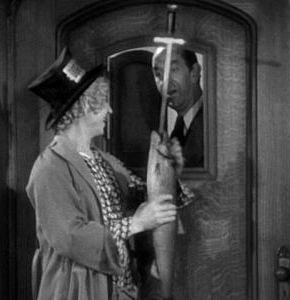
\includegraphics[width=.4\textwidth]{swordfish.jpg}
\end{center}

\end{frame}

\begin{frame}{Things you have}

\begin{itemize}
  \item USB device (token, thumb drive with data on it)
  \item driver's license
  \item passport
  \item a floppy disk, CD, DVD, or Blu-ray
  \item cell phone with a certain number
  \item computer already logged into your account
  \item pre-determined shared secret
  \item challenge coins
  \item credit cards
  \item a copy of a book
\end{itemize}
\end{frame}

\begin{frame}{Things you are}

\begin{itemize}
  \item biometrics
  \begin{itemize}
    \item fingerprints
    \item face
    \item retina
    \item signature
  \end{itemize}
  \item you are alive (blood flow, temperature)
  \item reasoning (CAPTCHA, Contact)
\end{itemize}
\end{frame}

\begin{frame}{2FA and MFA}

``MFA'' means multi-factor authentication.

\ \\

2FA means $M=2$.

\ \\

When you ``add 2FA,'' it almost universally means that you already have a password established and you are adding a ``thing you have'' factor, generally a phone number or a TOTP shared secret.

\end{frame}

\begin{frame}{SMS and Email}

SMS and email-based 2-factor auth are common, but not very secure.

\ \\

SMS and email are easily compromised and insecurely transmitted.

\ \\

Certainly \textbf{better than nothing}.

\ \\

But really try to do better.

\end{frame}

\begin{frame}{Apps}

Google Authenticator, Authy, Duo, and friends are more secure.

\ \\

Apps for iOS, Android, Blackberry.

\ \\

HOTP and TOTP are open protocols.

\end{frame}

\begin{frame}{HOTP}
HMAC-based one-time password (RFC 4226).

\ \\

HMAC means hash-based message authentication code (RFC 2104).

HMAC-SHA1 means we use SHA1 as our hashing algorithm.

\ \\

$\oplus$ means XOR.

$||$ means concatenation.

$C$ is an 8-byte counter (starts at 0).

$K$ is some shared secret.

\begin{multline*}
\text{HMAC}(K, m) = \text{SHA1}((K \oplus \texttt{0x5c5c}) \dots || \\ \text{SHA1}((K \oplus \texttt{0x3636}\dots) || m))
\end{multline*}

$$\text{HOTP}(K, C) = \text{Truncate}(\text{HMAC}(K, C))$$
\end{frame}

\begin{frame}[fragile]{HOTP in Python}

\begin{block}{HOTP}
\py
\begin{lstlisting}
xor_5c = "".join(chr(x ^ 0x5c) for x in xrange(256))
xor_36 = "".join(chr(x ^ 0x36) for x in xrange(256))
blocksize = hashlib.sha1().block_size

def hmac_sha1(key, msg):
    if len(key) > blocksize:
        key = hashlib.sha1(key).digest()
    key += chr(0) * (blocksize - len(key))
    o_key_pad = key.translate(xor_5c)
    i_key_pad = key.translate(xor_36)
    return hashlib.sha1(o_key_pad + hashlib.sha1(i_key_pad + msg).digest()).digest()
\end{lstlisting}
\end{block}
\end{frame}

\begin{frame}[fragile]{Truncate}

Truncate the HMAC-SHA1 result into a 6--8-digit number.

\ \\

6 is the most common number of digits.

\ \\

\begin{block}{HOTP}
\py
\begin{lstlisting}
def truncate(result, digits):
    offset = ord(hmac_result[19]) & 0xf
    num = ((ord(hmac_result[offset]) & 0x7f) << 24) \\
         | (ord(hmac_result[offset+1])       << 16) \\
         | (ord(hmac_result[offset+2])       <<  8) \\
         |  ord(hmac_result[offset+3])
    return num % (10**digits)
\end{lstlisting}
\end{block}
\end{frame}

\begin{frame}{TOTP}

TOTP (RFC 6238) is the same as HOTP, except the counter $C$ is based on time.

$$C = T = \lfloor(\texttt{time.time()} - T_0) / X\rfloor$$

\texttt{time.time()} is the number of seconds since the UNIX epoch.

\ \\

$T_0$ is generally $0$, meaning calculated relevant to the UNIX epoch.

\ \\

(The UNIX epoch is 1970-01-01T00:00:00Z.)

\ \\

Typically, $X = 30$ (so codes are valid for about 30 seconds).

\ \\

Division is floor-division.

\end{frame}

\begin{frame}{HOTP and TOTP Security}

How secure are these 6-digit numbers?

\ \\

\textbf{Reasonably} secure.

\ \\

Six digits $ = 1000000 \approx 2^{20}$.

\ \\

A typical password has about 21 bits of entropy.

\ \\

\textbf{Most importantly}, those 6 digits do not reveal anything meaningful about the underling secret. So you can leak as many of them as you like, and it will not help an attacker.

\ \\

Weaknesses in SHA1 have not affected the security of HOTP / TOTP.

\end{frame}

\begin{frame}{QR codes}

How do you transmit the secret? QR codes.

\ \\

How does a QR code work? That would be a whole extra talk.

\ \\

\url{otpauth://totp/swenson?secret=26FXII6KEZWOJWIAEI2PZSOXDCZBQHMR&algorithm=SHA1&digits=6&period=30}

\ \\

See \url{https://github.com/google/google-authenticator/wiki/Key-Uri-Format}

\begin{center}
  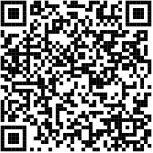
\includegraphics{qrcode.png}
\end{center}

\end{frame}

\begin{frame}{TPM}
Trusted Platform Module\,---\,basically like a built-in yubikey into your device or computer.

\ \\

Can store things as well as generate new keys in a way that no one can ever get the private key.

\ \\

Generally, a ``secure element'' and a standard set of protocols for accessing it.

\end{frame}

\begin{frame}{Django 2FA}

\texttt{pip install django-otp \&\& pip install qrcode}

\begin{itemize}
  \item Supports TOTP, HOTP, Email, (optionally) SMS, Yubikey
  \item Can hook into a normal login flow or the admin login flow easily
  \item A bit rough around the edges
  \item Flow is awkward.
  \item Admin can see secrets.
  \item No easy enrollment or reset.
\end{itemize}

(Sprint anyone?)

\end{frame}


\begin{frame}[fragile]{Django 2FA (cont'd.)}

\begin{block}{site settings.py}
\py
\begin{lstlisting}
INSTALLED_APPS = [
    'sampleapp.apps.OtpAdminConfig',  # replaces 'django.contrib.admin'
    'django_otp',
    'django_otp.plugins.otp_totp',
    'django_otp.plugins.otp_hotp',
    'django_otp.plugins.otp_static',
]
MIDDLEWARE = [
    'django_otp.middleware.OTPMiddleware',
]
\end{lstlisting}
\end{block}

Run migrations and all that jazz.

\ \\

\texttt{\$ python manage.py migrate}

\end{frame}


\begin{frame}[fragile]{Django 2FA (cont'd.)}

\begin{block}{app admin.py}
\py
\begin{lstlisting}
from django.contrib import admin
from django_otp.admin import OTPAdminSite

class OtpAdminSite(OTPAdminSite):
    pass
\end{lstlisting}
\end{block}
\end{frame}


\begin{frame}[fragile]{Django 2FA (cont'd.)}

\begin{block}{app apps.py}
\py
\begin{lstlisting}
from django.apps import AppConfig
from django.contrib.admin.apps import AdminConfig

class SampleappConfig(AppConfig):
    name = 'sampleapp'

class OtpAdminConfig(AdminConfig):
    default_site = 'sampleapp.admin.OtpAdminSite'
\end{lstlisting}
\end{block}
\end{frame}


\begin{frame}[fragile]{Django 2FA (cont'd.)}
Can use it like:
\begin{block}{app views.py}
\py
\begin{lstlisting}
from django.shortcuts import render, redirect
from django.http import HttpResponse

def index(request):
    if not (request.user.is_authenticated and request.user.is_verified()):
        return redirect('/admin/?next=%s' % (request.path))
    return HttpResponse("Hello, world!")
\end{lstlisting}
\end{block}
\end{frame}

\begin{frame}{Demo}
Time for a demo?
\end{frame}

\begin{frame}{Problems with MFA}
Lose your device $\Rightarrow$ you can be out of luck.

\ \\

Backup solutions (e.g., recover codes) are cumbersome.

\ \\

Hope that \emph{only} you can convince support to reset your account.

\ \\

Annoying to type in codes from devices.

\ \\

Bluetooth difficult to use with multiple accounts.

\ \\

Hardware can often only hold 1--3 sets of keys.

\ \\

HOTP and TOTP keys are symmetric\,---\,admin can impersonate you.


\end{frame}

\begin{frame}{U2F}

Universal 2-Factor, standardized by FIDO, jointly developed by Yubico and Google.

\ \\

Different communications allowed: USB, BT, NFC

\ \\

Based on ECDSA (RSA too in the latest spec).

\ \\

Designed to be inexpensive, easy-to-use, and relatively secure.

\ \\

Not well-supported outside of the largest websites.

\ \\

Django support is nearly non-existant. (Sprint anyone?)

\end{frame}

\begin{frame}

Take-aways:

\begin{itemize}
  \item Use an app if you can
  \item A hardware token is better
  \item Even better if it is U2F
  \item Try to integrate it into your system (carefully)!
\end{itemize}

I'm happy to take questions!

\end{frame}

\end{document}
% %sagemathcloud={"zoom_width":155}
